% -*- coding: utf-8; -*-
% vim: set fileencoding=utf-8 :
\documentclass[english,submission]{programming}
%% First parameter: the language is 'english'.
%% Second parameter: use 'submission' for initial submission, remove it for camera-ready (see 5.1)

\usepackage[backend=biber]{biblatex}
\addbibresource{reference.bib}
\usepackage{tikz}
\usepackage{listings}
\usepackage{graphicx}
\usepackage{subcaption} % For subfigures


%
% Packages and Commands specific to article (see 3)
%
% These ones  are used in the guide, replace with your own.
% 
\usepackage{multicol}
\lstdefinelanguage[programming]{TeX}[AlLaTeX]{TeX}{%
  deletetexcs={title,author,bibliography},%
  deletekeywords={tabular},
  morekeywords={abstract},%
  moretexcs={chapter},%
  moretexcs=[2]{title,author,subtitle,keywords,maketitle,titlerunning,authorinfo,affiliation,authorrunning,paperdetails,acks,email},
  moretexcs=[3]{addbibresource,printbibliography,bibliography},%
}%
\lstset{%
  language={[programming]TeX},%
  keywordstyle=\firamedium,
  stringstyle=\color{RosyBrown},%
  texcsstyle=*{\color{Purple}\mdseries},%
  texcsstyle=*[2]{\color{Blue1}},%
  texcsstyle=*[3]{\color{ForestGreen}},%
  commentstyle={\color{FireBrick}},%
}

\newcommand*{\CTAN}[1]{\href{http://ctan.org/tex-archive/#1}{\nolinkurl{CTAN:#1}}}
%%


%%%%%%%%%%%%%%%%%%
%% These data MUST be filled for your submission. (see 5.3)
\paperdetails{
  %% perspective options are: art, sciencetheoretical, scienceempirical, engineering.
  %% Choose exactly the one that best describes this work. (see 2.1)
  perspective=engineering,
  %% State one or more areas, separated by a comma. (see 2.2)
  %% Please see list of areas in http://programming-journal.org/cfp/
  %% The list is open-ended, so use other areas if yours is/are not listed.
  area={Live programming, language engineering},
  %% You may choose the license for your paper (see 3.)
  %% License options include: cc-by (default), cc-by-nc
  % license=cc-by,
}
%%%%%%%%%%%%%%%%%%

%%%%%%%%%%%%%%%%%%
%% These data are provided by the editors. May be left out on submission.
%\paperdetails{
%  submitted=2016-08-10,
%  published=2016-10-11,
%  year=2016,
%  volume=1,
%  issue=1,
%  articlenumber=1,
%}
%%%%%%%%%%%%%%%%%%
\definecolor{codegray}{gray}{0.9}
\newcommand{\code}[1]{\colorbox{codegray}{\texttt{#1}}}

\begin{document}

\title{Language-Parametric Techniques for Live Probes}
%\subtitle{Preparing Articles for Programming}% optional
%\titlerunning{Preparing Articles for Programming} %optional, in case that the title is too long; the running title should fit into the top page column

\author[a]{Jean-Baptiste Döderlein}
\affiliation[a]{ENS Rennes, Bruz, France}
\author[b]{Riemer van Rozen}
\affiliation[b]{Centrum Wiskunde \&\ Informatica (CWI), Amsterdam, The Netherlands}
\author[b,c]{Tijs van der Storm}
\affiliation[c]{University of Groningen, Groningen, The Netherlands}


\keywords{programming journal, paper formatting, submission preparation} % please provide 1--5 keywords


%%%%%%%%%%%%%%%%%%%%%%%%%%%%%
% Please go to https://dl.acm.org/ccs/ccs.cfm and generate your Classification
% System [view CCS TeX Code] stanz and copy _all of it_ to this place.
%% From HERE
\begin{CCSXML}
<ccs2012>
<concept>
<concept_id>10002944.10011122.10003459</concept_id>
<concept_desc>General and reference~Computing standards, RFCs and guidelines</concept_desc>
<concept_significance>300</concept_significance>
</concept>
<concept>
<concept_id>10010405.10010476.10010477</concept_id>
<concept_desc>Applied computing~Publishing</concept_desc>
<concept_significance>300</concept_significance>
</concept>
</ccs2012>
\end{CCSXML}

\ccsdesc[300]{General and reference~Computing standards, RFCs and guidelines}
\ccsdesc[500]{Applied computing~Publishing}

% To HERE
%%%%%%%%%%%%%%%%%%%%%%%

\maketitle

% Please always include the abstract.
% The abstract MUST be written according to the directives stated in 
% http://programming-journal.org/submission/
% Failure to adhere to the abstract directives may result in the paper
% being returned to the authors.
\begin{abstract}
  %What is the broad context of the work? What is the importance of the general research area?
  \textit{Context.}
  In the first part of his 2012 presentation ``Inventing on Principle''~\cite{InventingOnPrinciple}, Bret Victor gives a demo of live code editor for Javascript which shows the dynamic history of values of variables in real time. This form of live programming has become known as ``live probes''~\cite{MakingMethodsLive,UsableLiveProgramming,ExampleBasedGraalVM}. Using live probes the programmer has a permanent and continuous insight into the dynamic evolution of function or method variables, thus improving feedback and developer experience. 
  
  % What problem or question does the paper address? How has this problem or question been addressed by others (if at all)?
  \textit{Inquiry.} Although Bret Victor shows a working prototype of live probes in the context of Javascript, he does not discuss strategies for implementing them. Later work~\cite{ExampleBasedGraalVM} provides an implementation approach, but this requires a programming language to be implemented on top of the GraalVM runtime~\cite{GraalVM}. In this paper we investigate generic engineering strategies that can be applied in the context of many programming languages, without requiring dedicated compiler or runtime support. 
  
  % What was done that unveiled new knowledge?
  \textit{Approach.}
  In this paper we explore how debugger protocols can be exploited to implement live probes. Methods or functions are compiled after every code change and executed inside the debugger. During execution the evolution of all local variables in the current stack frame are recorded and communicated back to the IDE for display to the user. 

  % What new facts were uncovered? If the research was not results oriented, what new capabilities are enabled by the work?
  \textit{Knowledge.}
  It turns out that debugger protocols are rich enough for implementing live probes. Step-wise execution, hot code swapping and stack frame inspection provide the right granularity and sufficient information to realize live probes, without modifying compilers or language runtimes. Furthermore, it turns out that the recently proposed Debugger Adapter Protocol (DAP)~\cite{DAP} provides an even more generic approach of implementing live probes, but, in some cases, at the cost of a significant performance penalty. 

  % What argument, feasibility proof, artifacts, or results and evaluation support this work?
  \textit{Grounding.}
  We have implemented live probes using stack recording natively for Java through the Java Debug Interface (JDI)~\cite{JDI}, and through the DAP for Java, Python, C, and Javascript, all with minimum glue code.  We evaluate the run-time performance of all four live probes prototypes, decomposed into: compile-after-change, hotswap, single step overhead, and stack recording overhead. Our results show that live probes on top of native debugger APIs are performant enough for interactive use. In the case of DAP, it depends on characteristics of the programming language. 

  % Why does this work matter?
  \textit{Importance.} Live programming improves the programmer experience by providing immediate feedback about a program's execution and eliminating disruptive edit-compile-restart sequences. Live probes are one way to shorten the programmer feedback loop at the level of functions and methods. Although live probes are not new, and have been implemented in (prototype) systems, our approach of building live probes on top of existing and generic debugger protocols opens up live probes for a host of mainstream programming language, with minimum effort.
\end{abstract}

\section{Introduction}
\label{sec:introduction}

Live programming~\cite{TanimotoLevels,UsableLiveProgramming,ExampleCentric,Hancock03} promises a better programming experience by bringing the execution of a program closer to the abstractions of the source code. By erasing the distinction between a program on the one hand, and its execution on the other, programmers may enjoy a more fluid experience, with immediate dynamic feedback after every code change. 

Live programming has a rich history, both in academia and industrial research\footnote{For brief and incomplete overview of some of the history of live programming, see~\cite{LiveProgHist13}}, originating in the original Lisp systems (e.g.,~\cite{Sandewall78,Masinter81}) and Smalltalk~\cite{Goldberg80} which allowed dynamic replacement of code units (hot swapping) and inspection of program structures at run-time (sometimes referred to as ``programming in the debugger''). However, live programming became center stage after Bret Victor's influential talk ``Inventing on Principle'', which went viral in 2012. 

In that presentation Victor makes a compelling case that (paraphrasing) ``creators need to see what they are creating''. In the case of programming, this entails continuous inspection of the run-time behavior of a program, and immediate and seamless adaptation after a code change. While all the prototypes demonstrated by Victor are impressive, for the purpose of this paper we zoom in on one of them: a live editor for Javascript with a side pane showing the history of values of local function variables during an execution (see Figure~\ref{FIG:bret} below). Although not mentioned by Victor himself, this live programming features has become known as ``live probes''~\cite{UsableLiveProgramming,ExampleBasedGraalVM}.

The question left unanswered in Victor's presentation is: how to build such live probes? While there has been research showcasing implementation approaches~\cite{ExampleBasedGraalVM}, they depend on a specific runtime system (e.g., GraalVM), or employ language specific ``hacks''~\cite{LiveLiterals}, and hence cannot be easily transferred to other languages. So a more specific question is: how to  engineer live probes \textit{generically}, without dedicated compiler or runtime support?

In this paper we present an approach to implementing live probes reusing standard debugger protocols and APIs. Most language support an API to facilitate the implementation of debuggers and other run-time tools (e.g., profilers, tracers, etc.). It turns out that such facilities are sufficiently powerful for implementing live probes. The key to the approach is to (re)execute a function or method inside the debugger, step by step, and at each step record a snapshot of the current stack-frame. After the method has finished executing, the resulting stack recording is communicated back to the IDE and visualized alongside the code, matching stack recording entries to the source code using source location information.

We first detail how to implement live probes using a native debugger interface, the Java Debugger Interface (JDI). Then we generalize the approach to employ the recently proposed Debugger Adapter Protocol (DAP). 
This implementation is showcased with live probe implementations in Java (again), C, Python, and Javascript. 
As a result, live probes can be supported in any programming language that provides an implementation of the DAP, with only a limited amount of configuration code.  

Since live programming (and hence live probes) is all about immediate feedback, it is important that the performance overhead of our implementation strategy does not impede practical use. We therefore provide a detail analysis and measurement of the performance overhead of (re)compilation, hot-swapping, step-wise execution, and stack recording. To assess the overall usability of the approach, we furthermore decompose a full editing scenario (derived from Victor's presentation) in $X$ logical steps, replay it on every live probe implementation, and measure the performance of each step.

The contributions of this paper can be summarized as follows:
\begin{itemize}
  \item We analyze the requirements for implementing live probes (Section~\ref{sec:problem-overview})
  \item We introduce \textit{stack recording} as a technique to obtain the required information through standard debugger protocols (Section~\ref{sec:stack-recording})
  \item We implement live probes through stack recording on top of the Java Debugger Interface (JDI) (Section~\ref{sec:live-probes-java})
  \item We then generalize the approach via the Debugger Adapter Protocol (DAP) (Section~\ref{sec:generalizing-live-probes})
   \item We evaluate the feasibility of the approach by implementing live probes for Java, Python, C and Javascript on top the DAP, investigate the performance overhead of the individual steps, and reproduce an editing scenario to assess practicality (Section~\ref{sec:evaluation})
\end{itemize}

\section{Background and Overview}
\label{sec:problem-overview}


The basic concept of live probes is illustrated in Figure~\ref{FIG:bret}, showing two panes. 
The left pane shows an editor containing the source code of a possible implementation of binary search in Javascript. 
The right pane shows the values of variables matched up to the source line they were last updated.
The top two rows specify example input data that the function is executed on. The consecutive values of variables that are updated in a loop (e.g. \lstinline{low}, \lstinline{high}, \lstinline{mid} and \lstinline{value}) are displayed adjacently. So for \lstinline{low}, the history of values is 0, 3, and 5. Note that the update of \lstinline{high} in the else-if branch (apparently) never executed, so there is no (redundant) value display in the right pane. Finally, the last line shows the final return value of the function: apparently the \lstinline{key} was not found in the \lstinline[language=c]{array}. 

What makes this \textit{live} is that while the programmer is editing the program on the left (or the input arguments to the function), the value display on the right continuously updates so that it is apparent what is going on at run time. 


Dissecting this example leads to the following technical requirements for implementing live probes:
\begin{itemize}
  \item there should a way to specify the inputs to a method
  \item after every change to the code, it needs to be recompiled and reexecuted
  \item during execution the values of variables needs to be recorded and linked to source lines
  \item the resulting history list of values needs to be communicated to the IDE
\end{itemize}


The basic intuition of our approach to meet these requirements is as follows: a separate process, called the \textit{Keep Alive Agent} (KAA) starts the debugger in the background and monitors the editor for changes to the source code. Whenever the programmer edits the code, the KAA attempts to recompile the code, and, if successful, hotswaps the current method into the debugger. It then queries the source code for annotations (either explicit annotations as in Java, or special comments) specifying the input arguments to the method. The KAA then sets a breakpoint on the first statement of the method, and invokes it. Since there is a breakpoint, the debugger halts. Using the common step-over facility of a typical debugger, the KAA then steps through the whole method until its execution completes. During this process however, the KAA takes snapshots of the current stack frame to record the values of local variables. These snapshots are stored in a data structure, called \textit{stack recording}, which supports displaying the values in the IDE, for instance, like in Figure~\ref{FIG:bret}, inline~\cite{LiveLiterals,ExampleBasedGraalVM}, or using some other UI affordance. 



\begin{figure}[t]
  \centering
  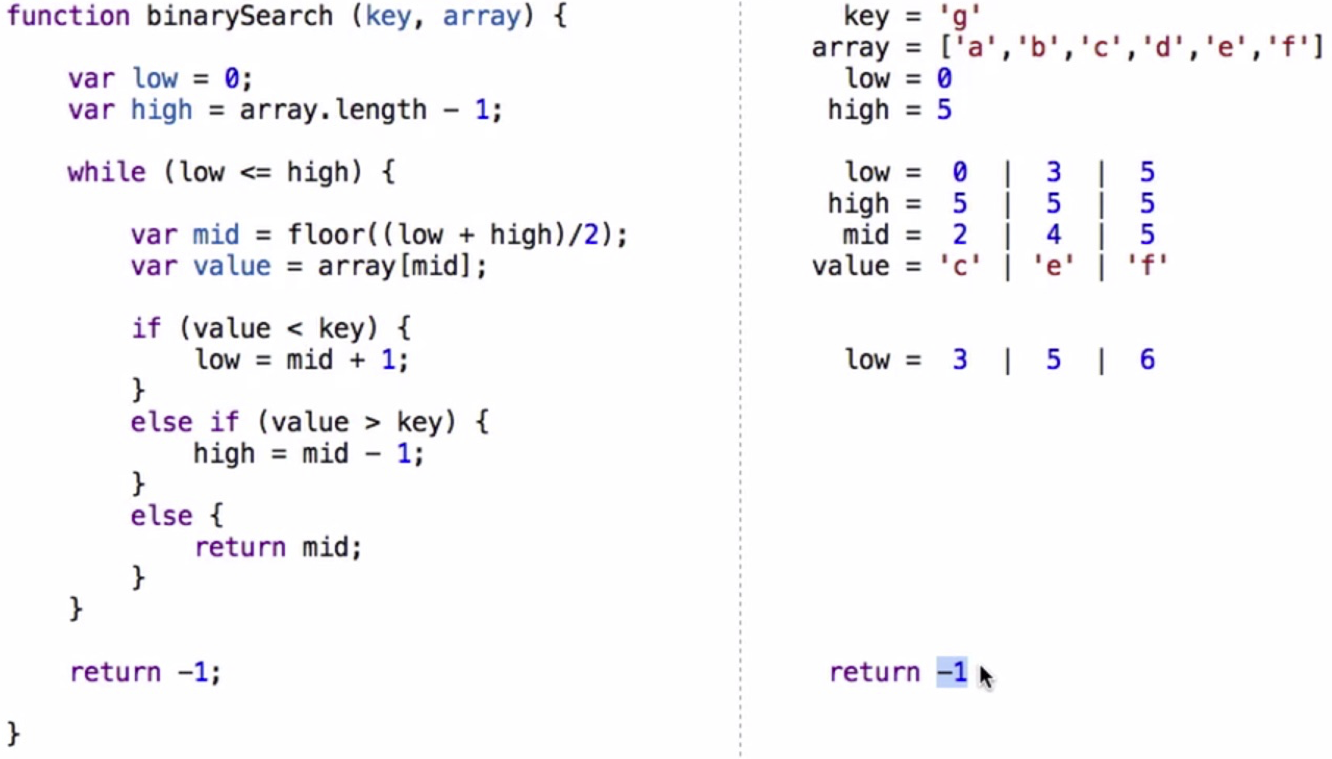
\includegraphics[width=\textwidth]{img/bret}
  \caption{Screenshot of Bret Victor's 2012 talk ``Inventing on Principle'' (23rd minute)}
  \label{FIG:bret}
\end{figure}


\section{Using the Debugger ?}

\subsection{Architecture}

\begin{figure}[h]
  \centering
  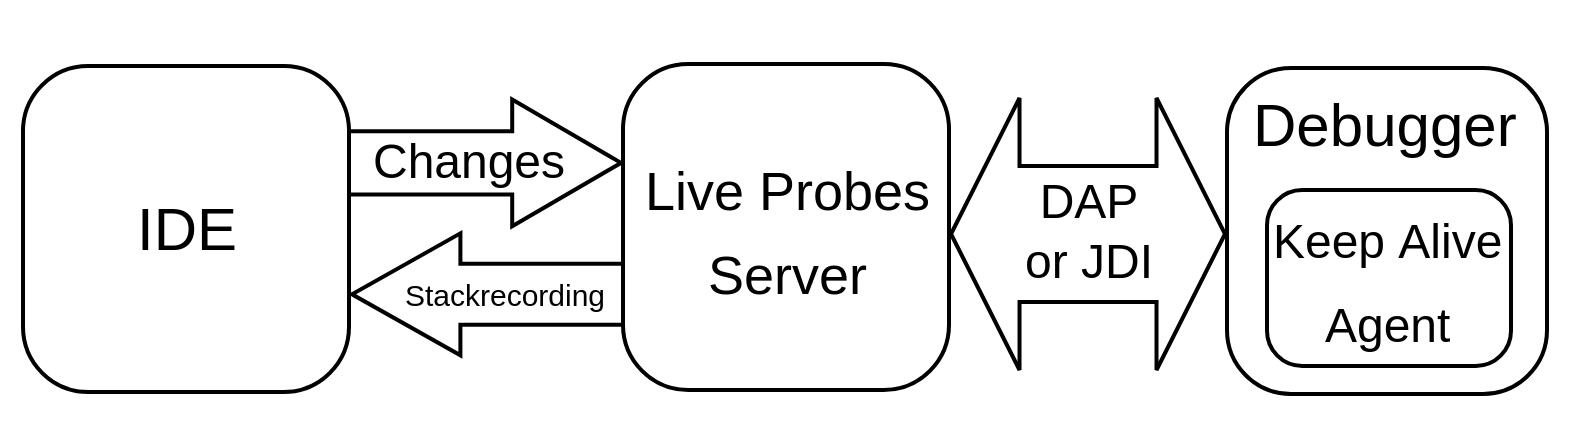
\includegraphics[width=0.8\linewidth]{img/architecture.png}
  \caption{General architecture (placeholder)}
  \label{fig:architecture}
\end{figure}

A live environment must be able to react to two different events: a change in the code or a change in the test/input data. 
If the code changes, we need to re-execute the code, and in the case of a compiled language, we need to compile the new code first. 
If the data changes, we need to be able to re-execute the programme with the new data. 
In addition, it is necessary to keep compilation and execution times low enough to maintain an interactive experience with the user.

To meet these constraints, we propose the architecture shown in Figure \ref{fig:architecture} :
\begin{itemize}
  \item The IDE or editor communicates with a server. The IDE sends changes to the code and function parameters, and the server sends back the stack trace of the method.
  \item The server initialises and communicates with the debugger to apply the changes received from the IDE, and generates a stack recording when the method is executed.
  \item The debugger runs an intermediate program, a keep alive agent. This keeps the debugger alive to reduce initialisation times.
\end{itemize}

\label{sec:stack-recording}

\subsection{Stack Recording}

\begin{figure}[h]
  \centering
  \begin{minipage}{0.2\textwidth}
    \begin{lstlisting}[language=C]
//foo(3)
int foo(int n) {
  int i = 0;
  while (i < n) {
    i++;
  }
  return i;
}
    \end{lstlisting}
  \end{minipage}
  \hfill
  \begin{minipage}{0.7\textwidth}
    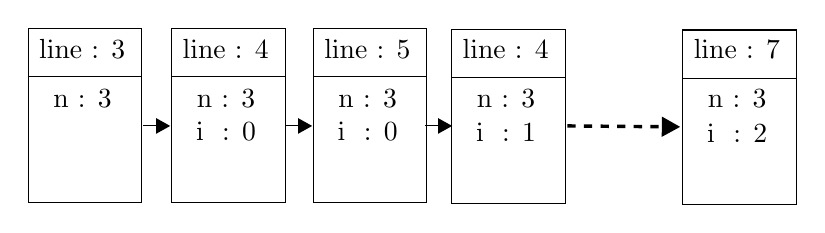
\begin{tikzpicture}[x=0.75pt,y=0.75pt,yscale=-1.1,xscale=0.95]
      
%Shape: Rectangle [id:dp48530454252997635] 
\draw   (11,13.3) -- (68.6,13.3) -- (68.6,34.5) -- (11,34.5) -- cycle ;
%Shape: Rectangle [id:dp4741172814816692] 
\draw   (11,34.5) -- (68.6,34.5) -- (68.6,89.7) -- (11,89.7) -- cycle ;
%Shape: Rectangle [id:dp39333640528563685] 
\draw   (83.8,13.3) -- (141.4,13.3) -- (141.4,34.5) -- (83.8,34.5) -- cycle ;
%Shape: Rectangle [id:dp852338699133017] 
\draw   (83.8,34.5) -- (141.4,34.5) -- (141.4,89.7) -- (83.8,89.7) -- cycle ;
%Shape: Rectangle [id:dp7978026394194542] 
\draw   (155.6,13.3) -- (213.2,13.3) -- (213.2,34.5) -- (155.6,34.5) -- cycle ;
%Shape: Rectangle [id:dp7423976709217543] 
\draw   (155.6,34.5) -- (213.2,34.5) -- (213.2,89.7) -- (155.6,89.7) -- cycle ;
%Shape: Rectangle [id:dp7923849318907303] 
\draw   (225.8,13.7) -- (283.4,13.7) -- (283.4,34.9) -- (225.8,34.9) -- cycle ;
%Shape: Rectangle [id:dp8325747263531937] 
\draw   (225.8,34.9) -- (283.4,34.9) -- (283.4,90.1) -- (225.8,90.1) -- cycle ;
%Shape: Rectangle [id:dp3066063334990279] 
\draw   (343,14.1) -- (400.6,14.1) -- (400.6,35.3) -- (343,35.3) -- cycle ;
%Shape: Rectangle [id:dp9425547748588214] 
\draw   (343,35.3) -- (400.6,35.3) -- (400.6,90.5) -- (343,90.5) -- cycle ;
%Straight Lines [id:da5537198175803346] 
\draw    (69.4,56.1) -- (80,56.1) ;
\draw [shift={(83,56.1)}, rotate = 180] [fill={rgb, 255:red, 0; green, 0; blue, 0 }  ][line width=0.08]  [draw opacity=0] (7.14,-3.43) -- (0,0) -- (7.14,3.43) -- cycle    ;
%Straight Lines [id:da9992180079914922] 
\draw    (141.4,56.1) -- (152,56.1) ;
\draw [shift={(155,56.1)}, rotate = 180] [fill={rgb, 255:red, 0; green, 0; blue, 0 }  ][line width=0.08]  [draw opacity=0] (7.14,-3.43) -- (0,0) -- (7.14,3.43) -- cycle    ;
%Straight Lines [id:da24526356738515775] 
\draw    (212.4,56.1) -- (223,56.1) ;
\draw [shift={(226,56.1)}, rotate = 180] [fill={rgb, 255:red, 0; green, 0; blue, 0 }  ][line width=0.08]  [draw opacity=0] (7.14,-3.43) -- (0,0) -- (7.14,3.43) -- cycle    ;
%Straight Lines [id:da7346663349503276] 
\draw [line width=1.25, dashed]    (284.4,56.1) -- (337.6,56.47) ;
\draw [shift={(341.6,56.5)}, rotate = 180.4] [fill={rgb, 255:red, 0; green, 0; blue, 0 }  ][line width=0.08]  [draw opacity=0] (9.29,-4.46) -- (0,0) -- (9.29,4.46) -- cycle    ;

% Text Node
\draw (15.2,17) node [anchor=north west][inner sep=0.75pt]   [align=left] {line : 3};
% Text Node
\draw (22.4,39) node [anchor=north west][inner sep=0.75pt]   [align=left] {n : 3};
% Text Node
\draw (88,17) node [anchor=north west][inner sep=0.75pt]   [align=left] {line : 4};
% Text Node
\draw (95.2,39) node [anchor=north west][inner sep=0.75pt]   [align=left] {n : 3};
% Text Node
\draw (94.8,53.2) node [anchor=north west][inner sep=0.75pt]   [align=left] {i \ : 0};
% Text Node
\draw (159.8,17) node [anchor=north west][inner sep=0.75pt]   [align=left] {line : 5};
% Text Node
\draw (167,39) node [anchor=north west][inner sep=0.75pt]   [align=left] {n : 3};
% Text Node
\draw (166.6,53.2) node [anchor=north west][inner sep=0.75pt]   [align=left] {i \ : 0};
% Text Node
\draw (230,17) node [anchor=north west][inner sep=0.75pt]   [align=left] {line : 4};
% Text Node
\draw (237.2,39) node [anchor=north west][inner sep=0.75pt]   [align=left] {n : 3};
% Text Node
\draw (236.8,53.6) node [anchor=north west][inner sep=0.75pt]   [align=left] {i \ : 1};
% Text Node
\draw (347.2,17) node [anchor=north west][inner sep=0.75pt]   [align=left] {line : 7};
% Text Node
\draw (354.4,39) node [anchor=north west][inner sep=0.75pt]   [align=left] {n : 3};
% Text Node
\draw (354,54) node [anchor=north west][inner sep=0.75pt]   [align=left] {i \ : 2};
    \end{tikzpicture}
  \end{minipage}
  \caption{Stack Recording Example}
  \label{fig:stack-recording}
\end{figure}

In order to generate the data needed to probe a variable, we need to be able to retrieve the state of the variable during execution. 
This information is contained in the stackframe at the time of execution. 
However, we need to add spatial and temporal information to this: we need to associate each stackframe state with the location in the code at which it was retrieved, and we also need to know the order in which these stackframes were retrieved.

In this paper, we introduce a structure for representing this data: a \textit{stack recording}. 
A stack record represents the different states of the stack frame during the execution of a method. The stack record is presented as a chain of recorded stack frames, to which information has been added about the source code's location and height in the stack.
This representation allows us to maintain a link between the spatial location (the reference to the source code) and the temporal location (the order of these stackframes) of the execution.
This representation has several advantages: it is easy to construct from debugger information, and it applies to most programming languages.
Figure \ref{fig:stack-recording} shows an example of a stack recording. On the left is a C function and on the right is the stack recording of the execution of \code{foo(3)}. Each rectangle represents the state of the stackframe during execution, with the source code location (here simplified to the line number).

\begin{figure}[h]
  \centering
  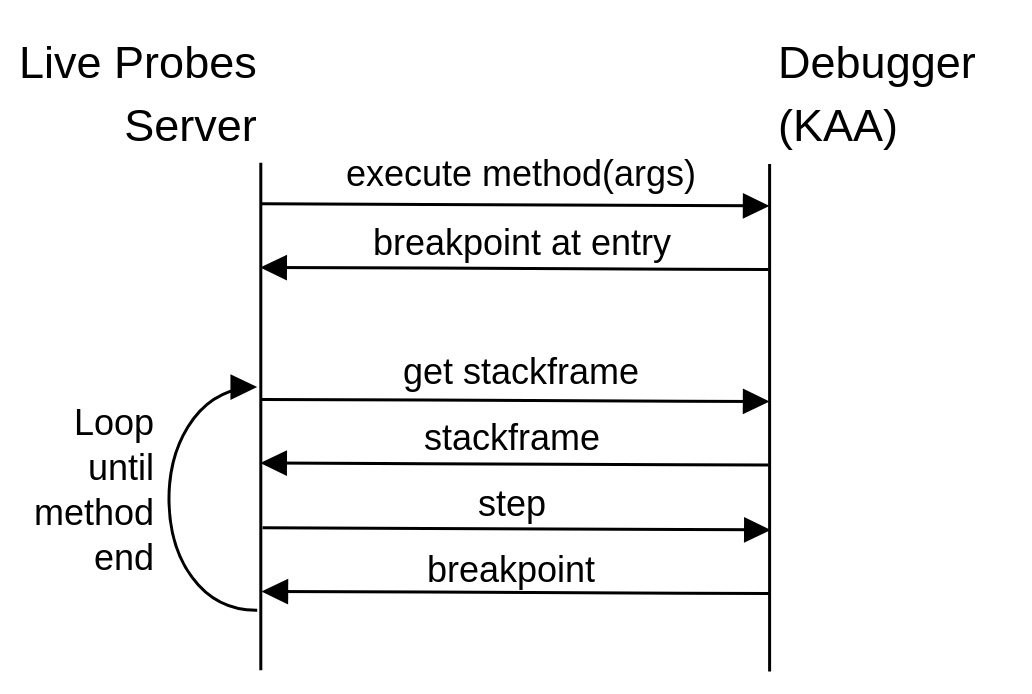
\includegraphics[width=0.6\linewidth]{img/stackrecording_impl.png}
  \caption{Record Stackrecording (placeholder)}
  \label{fig:stack-recording-impl}
\end{figure}

Figure \ref{fig:stack-recording-impl} shows how a stack recording is recorded.
To obtain the different states of the stackframe during the execution of a method, we place a breakpoint at the start of the function. 
Once this has been reached, the method is executed step by step, using the debugger's step instruction. 
Between each step, the state of the stackframe is recorded along with the source code's location information.


\section{Live Probes in Java with JDI}
\label{sec:live-probes-java}
% listing of a java class
\begin{figure}[htbp]
  \centering
  \begin{lstlisting}[language=Java]
public class Debugger{
  Debugger(){
    setBreakpointOnWhileTrue();
    launchVM(KeepeAliveAgent);
  }
  public void loadClass(classPath, className){
    addClassPathToDynamicClassLoader(classPath);
    loadClass(className);
  }

  public StackRecording execute(method, arguments){
    createMirrorArguments(arguments);
    setBreakpointAtMethod(method);
    invokeMethod(method, arguments);
    stackRecording = new StackRecording();
    while(!isMethodFinished()){
      stackRecording.add(getStackFrame());
      stepDebuggee();
    }
    return stackRecording;
  }
}
  \end{lstlisting}
  \caption{JDI Debugger classes}
  \label{fig:debugger-class}
\end{figure}

\begin{figure}[htbp]
  \centering
  \begin{lstlisting}[language=Java]
public class KeepAliveAgent {
  DynamicClassLoader dynamicClassLoader;

  public void loadClass(String className){
    dynamicClassLoader.loadClass(className);
  }

  public static void main(String[] args){
    while (true) {}
  }
}
  \end{lstlisting}
  \caption{JDI Keep Alive Agent}
  \label{fig:java-keep-alive-agent}
\end{figure}

We have developed a debugger capable of stack recording using JDI, a debugging interface for Java. 
A simplified pseudo code of this class is presented in Figure \ref{fig:debugger-class}.
The class includes a method to initialise the JVM (line 2), a method to search or reload a class in the VM (line 5) and a method to generate a stack recording of a method (line 10). 

For initialisation, a JVM containing the instrumentation provided by JDI is launched on the KeepAliveAgent class \ref{fig:java-keep-alive-agent} and a breakpoint is set on the infinite loop in the \code{main} function (line 9). 
This breakpoint is used to keep the debugger alive in a wait state, which is necessary to use the JDI primitives \code{mirrorOf}, \code{newInstance} and \code{invokeMethod}.

To load a class, we use a dynamic ClassLoader which allows us to add class paths and load a class during execution. 
When the code changes, the class is reloaded into the KeepAliveAgent. 
This method has one limitation: it only works if the class signature has not changed, and only the contents of the methods have changed. 
If the structure has changed, the KeepAliveAgent must be restarted. 
This limitation can be overcome with certain JVM implementations\cite{KABANOV201151}.

To execute the target method (line 10 in Debugger\ref{fig:debugger-class}), the arguments are created in the client JVM, then passed to the debugger JVM using the \code{mirrorOf} and \code{newInstance} methods of the reflection API (line 11). 
A breakpoint is then placed at the input of the target method (line 12).
The target method is invoked using \code{invokeMethod}. 
Stack recording is then performed using the algorithm described in the previous paragraph. 
As long as the method is not finished, the debugger registers the stackframe and takes a step in the debuggee.

\section{Generalizing Live Probes with Debugger Adapter Protocol}
\label{sec:generalizing-live-probes}
The Debug Adapter Protocol (DAP), developed by Microsoft, is a standard method of communicating with a programming language debugger. It is compatible with various editors, including VS Code, and provides a unified interface for all programming languages. 

By exploiting this protocol, we have created a new language parametric backend, which we have implemented for the C, Python and Java programming languages. These languages are chosen to cover both compiled and interpreted languages. 
This backend offers an interface common to all three languages, which includes methods for starting and initialising the debugging server, loading and reloading code in the debugger, and executing a method while performing stack recording. 

These methods allow us to carry out stack recording independently of the chosen language and facilitate the future implementation of live programming interfaces. 

The implementation for each language includes a keep-alive agent and code to communicate with the debugger and keep-alive agent to provide the interface functionality.
These methods depend on both the implementation of the debugging server and the keep-alive agent. 
The debug server initialisation parameters are specific to each language.

The way in which the code is loaded also depends on the language. 
For interpreted languages such as Python, the code can be interpreted at runtime and then loaded into the debugger's memory. 
For Java, we have extended the ClassLoader to add and modify classpaths and classes at runtime in the keep-alive agent. 
For C, the code is loaded into shared libraries that can be added and reloaded during execution.

Method execution for Java and Python is different to that used in C. 
For Java and Python, calling methods directly from the debugger does not trigger breakpoints for these languages. 
To remedy this, execution must be initiated from the agent and not by a debugger command. 
To do this, the Python and Java agents have fields for referencing a method and its arguments; when this information is entered, the agent starts execution.
For C, as is the case in the backend using JDI, the method call is made from the debugger console.

\section{Evaluation}
\label{sec:evaluation}
\subsection{Demo : A Minimal Live Programming Environment}
\label{sec:demo-small-c}
\begin{figure}[htbp]
  \centering
  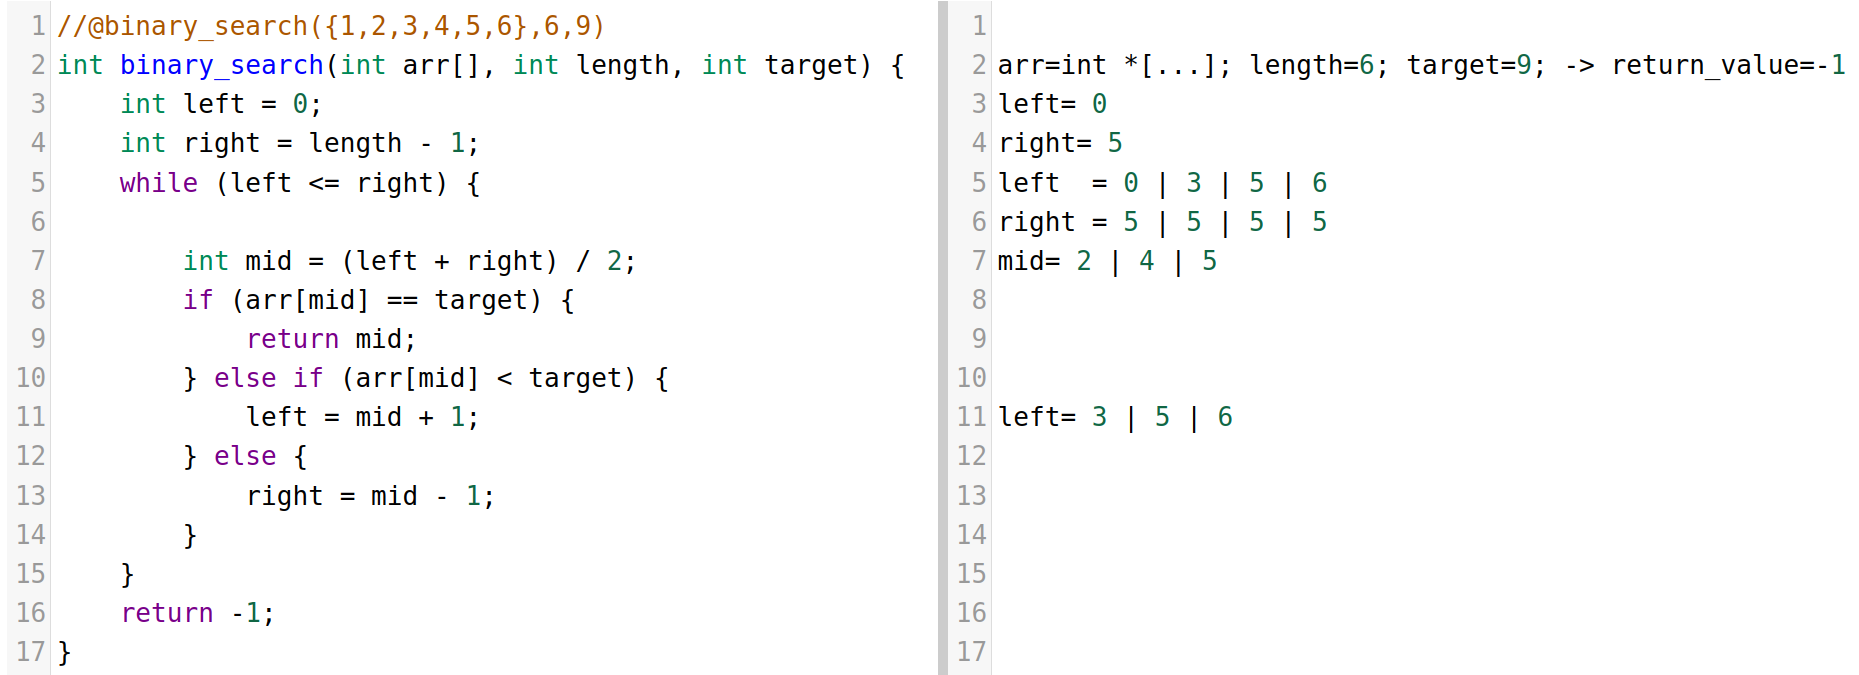
\includegraphics[width=\linewidth]{img/demo/c.png}
  \caption{Demo of the live programming environment for C.}
  \label{fig:demo}
\end{figure}

We have developed a dynamic programming environment that incorporates live probes through Java, C, and Python debug servers. 
The user interface consists of a web page that interacts with a local server. 
In Figure \ref{fig:demo}, we present a screenshot depicting a session with a binary\_search function in C. 
On the left-hand side, there is a code editor (based on CodeMirror 5), while on the right, a panel showcases live probes.

Whenever changes are made in the code editor, the code is sent to the server, which then checks for parseability and syntax errors. 
Additionally, if the code contains a comment starting with "@", followed by a function call, the server attempts to create a stack recording of that function, along with the provided parameters. 
This stack recording is subsequently processed through a parser to generate live probes, offering the following functionalities:

\begin{itemize}
  \item Displaying input arguments and return values for each function call.
  \item Showing the value of each variable definition or assignment. In cases where the assignment is within a loop or called multiple times, all the different values are displayed.
  \item Presenting the comparison values for each loop (for and while).
\end{itemize}
    
\subsection{Performance}
\label{sec:performance}

In the context of a live programming environment, it is essential to have short response times after user interactions. 
We therefore measured the performance of our approach in response to various questions:

\begin{itemize}
  \item How long does it take to compile and to load the code into the debugger, depending on the size of the programme?
  \item How long does it take to run the program, depending on the number of stack frames needed to make the stack recording?
  \item What is the average performance during a live programming session?
\end{itemize}

\subsubsection{How long does it take to compile and to load the code into the debugger, depending on the size of the programme?}

\begin{figure}[htbp]
  \centering
  \begin{subfigure}[b]{0.48\textwidth}
      \centering
      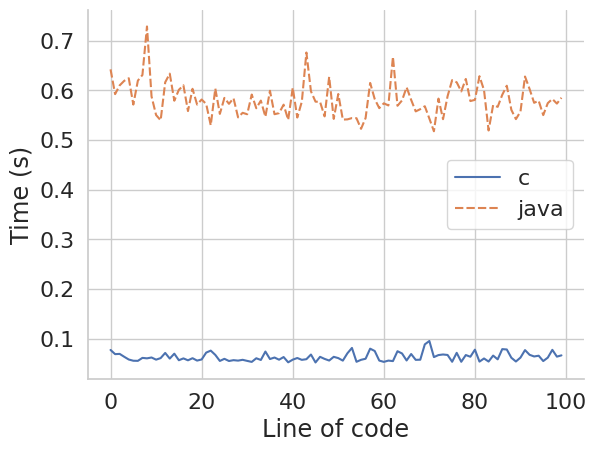
\includegraphics[width=\textwidth]{img/compile_code.png}
      \caption{\centering Compile code time}
      \label{subfig:compile}
  \end{subfigure}
  \hfill
  \begin{subfigure}[b]{0.48\textwidth}
      \centering
      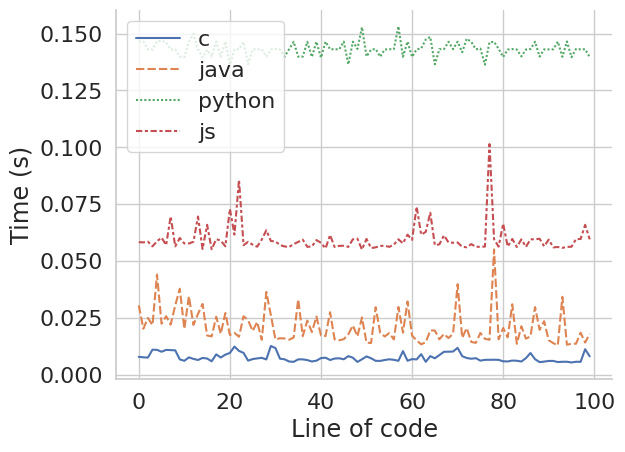
\includegraphics[width=\textwidth]{img/load_code.png}
      \caption{\centering Load code time}
      \label{subfig:load}
  \end{subfigure}
  \caption{Compile and load code time depending on the number of lines of code.}
  \label{fig:compileload}
\end{figure}

In our evaluation, we assessed the time required to compile and load code into the debugger memory for Python, C, and Java. 
To accomplish this, we compiled and loaded programs ranging from 5 to 100 lines of code. 
The summarized results can be found in Figure \ref{fig:compileload}.

In Sub-figure \ref{subfig:compile}, we present the compilation time for C and Java based on the number of lines of code. 
The compilation process was executed from the command line using javac and gcc. 
The compilation times remain nearly constant, regardless of the number of lines of code, with an average of 34.6 ms for Java and 8.5 ms for C.

Moving to Sub-figure \ref{subfig:load}, we depict the loading time in the debugger for C, Java, and Python as a function of the number of lines of code. 
The data shows that the loading time remains constant concerning the number of lines of code. 
On average, Python takes 3 ms, Java takes 2.8 ms, and C takes 1 ms for loading.

\subsubsection{How long does it need to run the program, depending on the number of steps to make the stack recording ?}

\begin{figure}[htbp]
  \centering
  \begin{subfigure}[b]{0.45\textwidth}
      \centering
      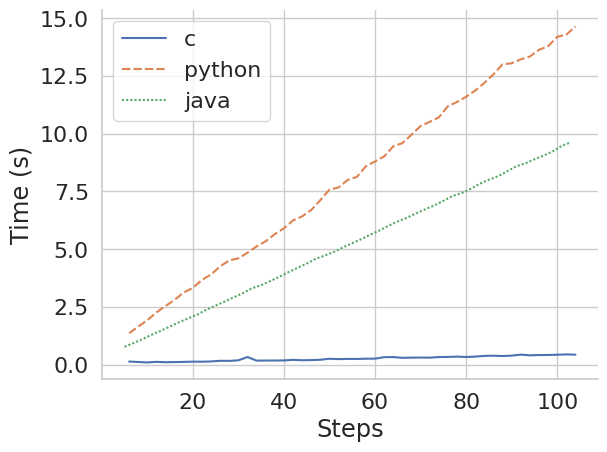
\includegraphics[width=\textwidth]{img/execute.png}
      \caption{\centering Total execution time}
      \label{subfig:execute-time-total}
  \end{subfigure}
  \hfill
  \begin{subfigure}[b]{0.45\textwidth}
      \centering
      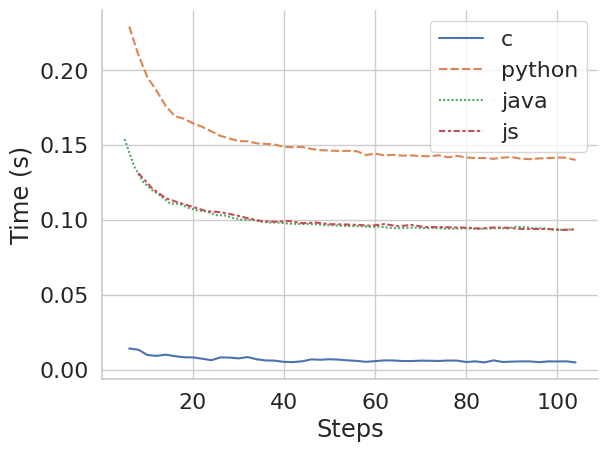
\includegraphics[width=\textwidth]{img/execute_ps.png}
      \caption{\centering Execution time per step}
      \label{subfig:execute-time-ps}
  \end{subfigure}
  \caption{Execution time in seconds depending on the number of steps.}
  \label{fig:execute-time}
\end{figure}

Subsequently, we proceeded to evaluate the execution time concerning the number of steps in the debugger. 
Figure \ref{subfig:execute-time-total} presents the total time taken based on the number of steps during stack recording, while Figure \ref{subfig:execute-time-ps} demonstrates the time per step as a function of the number of steps. 
Notably, the execution time exhibits a linear relationship with the number of steps in the method.

\subsubsection{What is the average performance during a live programming session?}

\begin{comment}
\begin{table}[h]
  \centering
  \begin{tabular}{@{} r c c c c c c c c c @{}}
  \toprule
  & \multicolumn{1}{c}{One time} & \multicolumn{3}{c}{Each Iteration} \\
  
  Language & Initialization & Compile & Load Code & Execute \\ \midrule
  C & 1.24 & 0.067 & 0.0098 & 0.193 \\
  Java & 5.92 & 0.57 & 0.015 & 1.28 \\
  Python & 0.639 & 0 & 0.144 & 3.26 \\
  \bottomrule
  \end{tabular}
  \caption{Average time in seconds for each step of the live programming session.}
  \label{table:average-time}
\end{table}

To evaluate the performance of our approach in the general context of a live programming session, we measured the times taken by the different stages of the interaction loop:

\begin{itemize}
  \item Agent initialisation time, which occurs once at the start of the session.
  \item The compilation time, if there is a compilation stage.
  \item The time taken to load the code into the debugger.
  \item Program execution time.
\end{itemize}

For the 3 languages we have implemented, we have performed the measurements for the execution of a binary search function \ref{fig:binary-search}.
For each language, the agent was initialized, then the code was compiled, loaded into the debugger and executed (with the array [1,2,3,4,5,6] and target 9) 100 times.
Each execution generate a stack recording of approximately 20 stack frames.
The results are shown in table \ref{table:average-time}.
\end{comment}
\begin{figure}[htbp]
  \centering
  \begin{subfigure}[b]{0.3\textwidth}
      \centering
      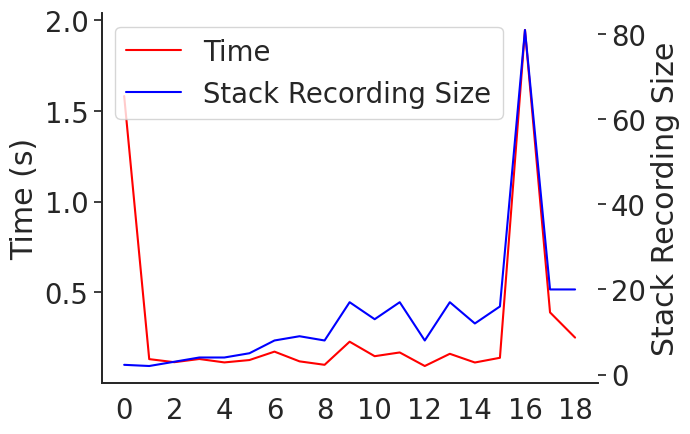
\includegraphics[width=\textwidth]{img/scenario_bs_c.png}
      \caption{\centering C}
      \label{subfig:scenario-bs-c}
  \end{subfigure}
  \hfill
  \begin{subfigure}[b]{0.3\textwidth}
      \centering
      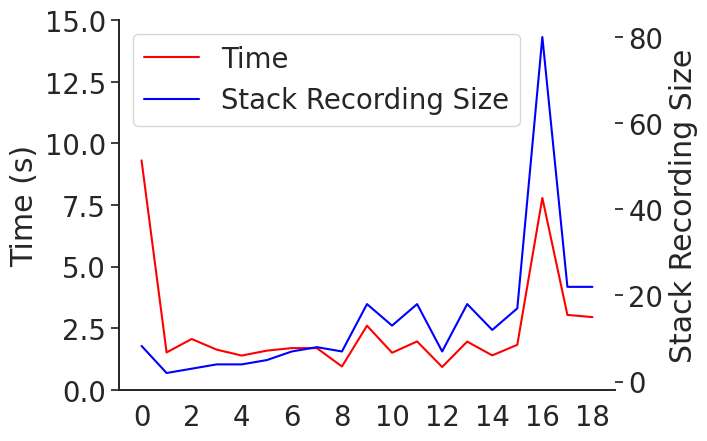
\includegraphics[width=\textwidth]{img/scenario_bs_java.png}
      \caption{\centering Java}
      \label{subfig:scenario-bs-java}
  \end{subfigure}
  \hfill
  \begin{subfigure}[b]{0.3\textwidth}
    \centering
    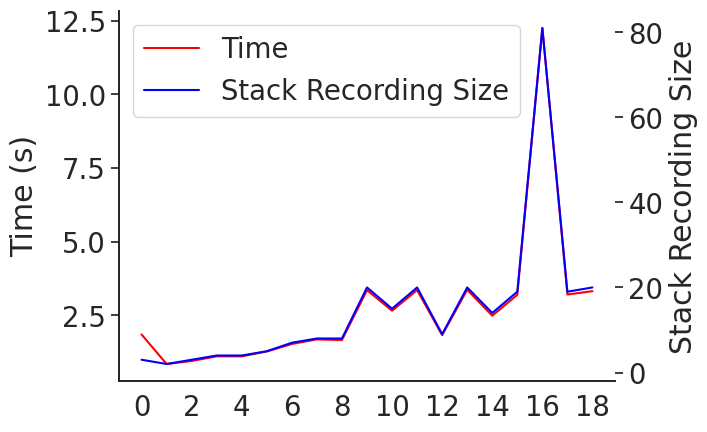
\includegraphics[width=\textwidth]{img/scenario_bs_python.png}
    \caption{\centering Python}
    \label{subfig:scenario-bs-py}
  \end{subfigure}

  \caption{Execution time and Stackrecording size for binary search scenario.}
  \label{fig:scenario-bs}
\end{figure}


To test the performance of our approach under real conditions, we recreated the live programming scenario presented in the video by bret victor. 
The scenario describes the programming of a function performing a binary search on an array of characters. It consists of 19 steps, including 10 steps where the source code is modified and 9 steps where the parameters are changed. 

\begin{enumerate}
  \item The function is defined and the parameters are defined to be an array of characters(\code{['a','b','c','d','e',f']}) and a target character(\code{'d'}).
  \item A new variable \code{low} is defined.
  \item A new variable \code{high} is defined.
  \item A new variable \code{mid} is defined.
  \item The variable \code{mid} is changed to be a integer.
  \item A new variable \code{value} is defined.
  \item A if and else snippets is added.
  \item The target is changed to \code{'b'}.
  \item The target is changed to \code{'c'}.
  \item The target is changed to \code{'d'} and the code from the \code{mid} is refactored to be in a \code{while(true)} loop.
  \item The target is changed to \code{'a'}.
  \item The target is changed to \code{'b'}.
  \item The target is changed to \code{'c'}.
  \item The target is changed to \code{'d'}.
  \item The target is changed to \code{'e'}.
  \item The target is changed to \code{'f'}.
  \item The target is changed to \code{'g'}.
  \item The condition of the while loop is changed to \code{low <= high}.
  \item A return \code{-1} is added at the end of the function.
\end{enumerate}


The scenario also includes the case where the tested method does not finish at step 17. As the code in Bret Victor's presentation is in Javascript, it has been adapted to the 3 languages studied in this paper.

For this test we set the maximum size of the stack recording at 80 stackframes. When the recording exceeds this limit, the debugger is stopped and restarted.

The figure \ref{fig:scenario-bs} shows the time and number of stackframes recorded for each stage of the scenario in Python, C and Java. 
When the initialisation is executed for Java and C, the time taken at each stage follows the same trend as the number of stack frames registered. 
At step 16, we also observe the case of an infinite loop in the scenario.


\section{Related Work}
\label{sec:related-work}

Example-Based Live Programming for Everyone\cite{ExampleBasedGraalVM} : Use GraalVM/Truffle to get live information from the code of multiple languages.

Example Centric Programming\cite{ExampleCentric} : Use BeanShell(custom JVM) to get live information. Prototype for Java in Eclipse.

Usable Live Programming\cite{UsableLiveProgramming} : New language for live programming(Ying Yang) with incremental compilation. Live programming environment for this language.
Use source location to relate execution and code(=> almost like stack recording that link stackframe and code location)

Scalable Omniscient Debugging\cite{ScalableOmniscient} : Omniscient debugging with a lot of data. Use a lot of memory to store all the data.
In this paper they record almost everything, we only record the stackframe.

LiveLiterals~\cite{LiveLiterals}

\section{Conclusion}
\label{sec:conclusion}

\printbibliography

\end{document}

% Local Variables:
% TeX-engine: luatex
% End:
